\documentclass[spanish,a4paper,12pt,oneside]{extreport}

\usepackage[dvips]{graphicx}
\usepackage[dvips]{epsfig}
\usepackage[utf8]{inputenc}
\usepackage[spanish]{babel}
\usepackage{alltt}

\usepackage[ruled,vlined,commentsnumbered,linesnumbered,inoutnumbered,titlenotnumbered,noend]{algorithm2e}
\SetKwRepeat{Do}{do}{while}

\usepackage{multirow}
\usepackage{array} 
\usepackage{amsfonts}
\usepackage{amsmath}
\usepackage{bigstrut}
\usepackage{booktabs}
\usepackage{caption}
\usepackage{chngpage}
\usepackage{float}
\usepackage{enumitem,lipsum}
\usepackage{graphicx}
\usepackage{lscape}
\usepackage{microtype}
\usepackage{natbib}
\usepackage{pdflscape}
\usepackage{rotating}
\usepackage{subcaption}
\usepackage{ctable}
\usepackage[hidelinks]{hyperref}
%\usepackage{enumerate}
\usepackage{gensymb}
\usepackage{eurosym}
\usepackage{xcolor}
\usepackage{tabu}

\usepackage{lineno}
%\\linenumbers
%\setlength\linenumbersep{5pt}
%\renewcommand\linenumberfont{\normalfont\tiny\sffamily\color{gray}}

\usepackage[top=2cm, bottom=2cm, left=2cm, right=2cm]{geometry}

\newenvironment{sourcecode}
{\begin{list}{}{\setlength{\leftmargin}{1em}}\item\scriptsize\bfseries}
{\end{list}}

\newenvironment{littlesourcecode}
{\begin{list}{}{\setlength{\leftmargin}{1em}}\item\tiny\bfseries}
{\end{list}}

\newenvironment{summary}
{\par\noindent\begin{center}\textbf{Abstract}\end{center}\begin{itshape}\par\noindent}
{\end{itshape}}

\newenvironment{keywords}
{\begin{list}{}{\setlength{\leftmargin}{1em}}\item[\hskip\labelsep \bfseries Keywords:]}
{\end{list}}

\newenvironment{palabrasClave}
{\begin{list}{}{\setlength{\leftmargin}{1em}}\item[\hskip\labelsep \bfseries Palabras clave:]}
{\end{list}}

\usepackage{bera}% optional: just to have a nice mono-spaced font
\usepackage{listings}
\usepackage{xcolor}

\colorlet{punct}{red!60!black}
\definecolor{background}{HTML}{EEEEEE}
\definecolor{delim}{RGB}{20,105,176}
\colorlet{numb}{magenta!60!black}

\lstdefinelanguage{json}{
    basicstyle=\normalfont\ttfamily,
    numbers=left,
    numberstyle=\scriptsize,
    stepnumber=1,
    numbersep=8pt,
    showstringspaces=false,
    breaklines=true,
    frame=lines,
    backgroundcolor=\color{background},
    literate=
     *{0}{{{\color{numb}0}}}{1}
      {1}{{{\color{numb}1}}}{1}
      {2}{{{\color{numb}2}}}{1}
      {3}{{{\color{numb}3}}}{1}
      {4}{{{\color{numb}4}}}{1}
      {5}{{{\color{numb}5}}}{1}
      {6}{{{\color{numb}6}}}{1}
      {7}{{{\color{numb}7}}}{1}
      {8}{{{\color{numb}8}}}{1}
      {9}{{{\color{numb}9}}}{1}
      {:}{{{\color{punct}{:}}}}{1}
      {,}{{{\color{punct}{,}}}}{1}
      {\{}{{{\color{delim}{\{}}}}{1}
      {\}}{{{\color{delim}{\}}}}}{1}
      {[}{{{\color{delim}{[}}}}{1}
      {]}{{{\color{delim}{]}}}}{1},
}

\begin{document}

\renewcommand\listtablename{Índice de Tablas}    
\renewcommand\listfigurename{Índice de Figuras}    

%%%%%%%%%%%%%%%%%%%%%%%%%%%%%%%%%%%%%%%%%%%%%%%%%%%%%%%%%%%%%%%%%%%%%%%%%%%%%%%
% First Page
%%%%%%%%%%%%%%%%%%%%%%%%%%%%%%%%%%%%%%%%%%%%%%%%%%%%%%%%%%%%%%%%%%%%%%%%%%%%%%%
\pagestyle{empty}
\thispagestyle{empty}


\newcommand{\HRule}{\rule{\linewidth}{1mm}}
\setlength{\parindent}{0mm}
\setlength{\parskip}{0mm}

\vspace*{\stretch{0.5}}

\begin{center}

\includegraphics[scale=0.8]{images/escuela-ingenieria-tecnologia-original}\\[10mm]
{\Huge Informe de la Práctica 7 de DAA \\[3mm] Curso 2023-2024}
\end{center}

\HRule
\begin{flushright}
        {\Huge \itshape Parallel Machine Scheduling Problem \\ with Dependent Setup Times} \\[5mm]
        {\Large NOMBRE ESTUDIANTE} \\[5mm]


\end{flushright}
\HRule
\vspace*{\stretch{2}}
\begin{center}
  \Large La Laguna, \today
\end{center}

\setlength{\parindent}{5mm}

\newpage
La Figura \ref{fig:PMSP} muestra una imagen creada por Midjourney recreando un ejemplo de aplicación real del problema abordado en esta práctica.

\begin{figure}
    \centering
    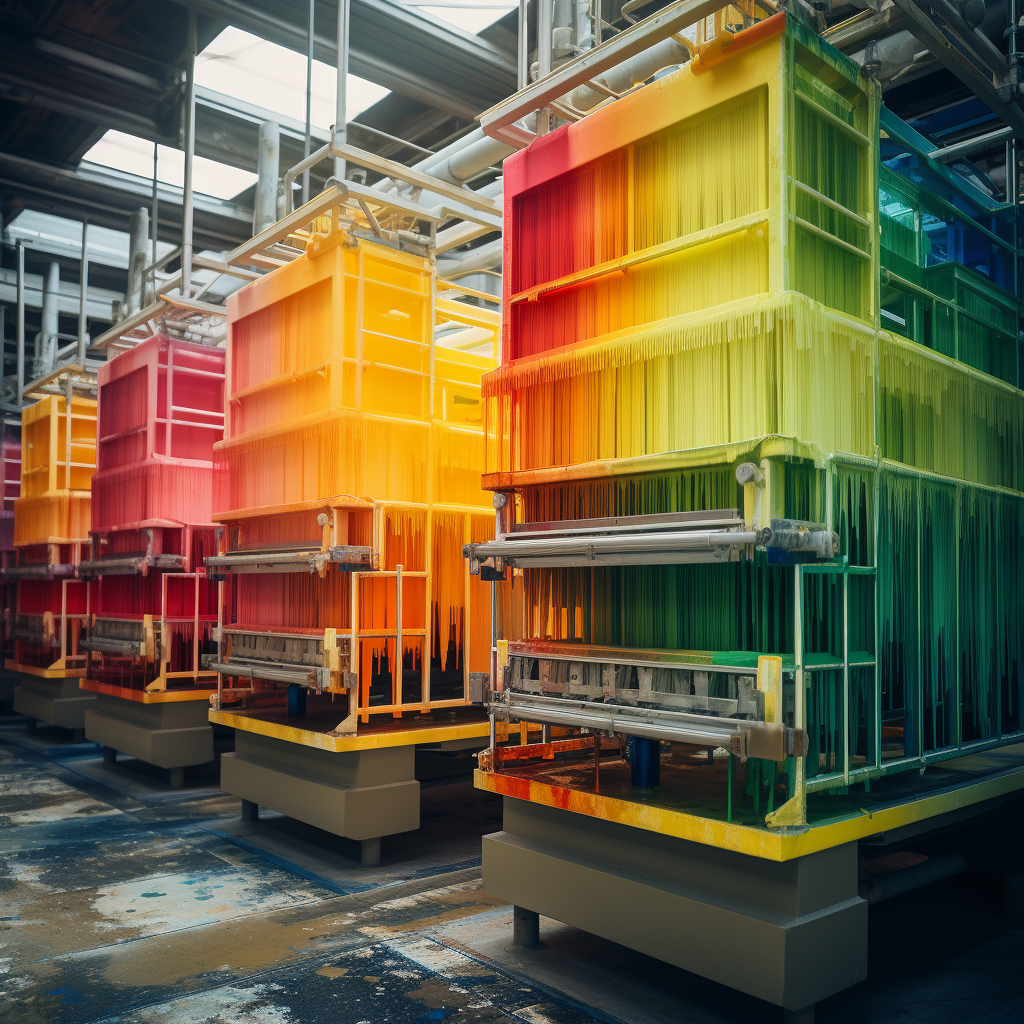
\includegraphics[scale=0.4]{images/PMSP_Midjourney.png}
    \caption{Midjourney}
    \label{fig:PMSP}
\end{figure}

%%%%%%%%%%%%%%%%%%%%%%%%%%%%%%%%%%%%%%%%%%%%%%%%%%%%%%%%%%
\newpage
\thispagestyle{empty}

{ \flushright

\begin{LARGE}
Agradecimientos
\end{LARGE}

\hspace{3mm}

\begin{large}
¿:-)?

\bigskip

\end{large}

}
%%%%%%%%%%%%%%%%%%%%%%%%%%%%%%%%%%%%%%%%%%%%%%%%%%%%%%%%
\newpage
\thispagestyle{empty}

\bigskip
\begin{LARGE}
Licencia
\end{LARGE}

\begin{center}
\includegraphics[scale=1.8]{images/by-nc_88x31}\\[5mm]
\end{center}

\begin{large}
© Esta obra está bajo una licencia de Creative Commons Reconocimiento-NoComercial 4.0 Internacional.
\end{large}

%%%%%%%%%%%%%%%%%%%%%%%%%%%%%%%%%%%%%%%%%%%%%%%%%%%%%%%%
\newpage
\thispagestyle{empty}

%%%%%%%%%%%%%%%%%%%%%%%%%%%%%%%%%%%%%%%%%%%%%%%%%%%%%%%%
\newpage 
\thispagestyle{empty}

\begin{abstract}
{\em

Resumen del trabajo realizado
}

\bigskip

\begin{palabrasClave}
Scheduling optimization problem, Total Completion Time, GRASP, LS, VNS. 
\end{palabrasClave}


\end{summary}
%%%%%%%%%%%%%%%%%%%%%%%%%%%%%%%%%%%%%%%%%%%%%%%%%%%%%%%%%
\newpage{\pagestyle{empty}}
\thispagestyle{empty}

%%%%%%%%%%%%%%%%%%%%%%%%%%%%%%%%%%%%%%%%%%%%%%%%%%%%%%%%%
\pagestyle{myheadings} %my head defined by markboth or markright
% No funciona bien \markboth sin "twoside" en \documentclass, pero al
% ponerlo se dan un montón de errores de underfull \vbox, con lo que no se
% ha puesto.


%%Aqui debería poner el nombre del proyecto pero, como es muy grande no cabe y se ve feo en el PDF
\markboth{xxxxx}{}

%%%%%%%%%%%%%%%%%%%%%%%%%%%%%%%%%%%%%%%%%%%%%%%%%%%%%%%%%
%Numeracion en romanos
\renewcommand{\thepage}{\roman{page}}
\setcounter{page}{1}
\pagestyle{plain} 

%%%%%%%%%%%%%%%%%%%%%%%%%%%%%%%%%%%%%%%%%%%%%%%%%%%%%%%%%

\tableofcontents

%%%%%%%%%%%%%%%%%%%%%%%%%%%%%%%%%%%%%%%%%%%%%%%%%%%%%%%%%
\newpage{\pagestyle{empty}}

\listoffigures

%%%%%%%%%%%%%%%%%%%%%%%%%%%%%%%%%%%%%%%%%%%%%%%%%%%%%%%%%
\newpage{\pagestyle{empty}}

\listoftables

%%%%%%%%%%%%%%%%%%%%%%%%%%%%%%%%%%%%%%%%%%%%%%%%%%%%%%%%%%%%%%%%%%%%%%%%%%%%%%%
\newpage{\pagestyle{empty}}

%%%%%%%%%%%%%%%%%%%%%%%%%%%%%%%%%%%%%%%%%%%%%%%%%%%%%%%%%%%%%%%%%%%%%%%%%%%%%%%
\newpage
\thispagestyle{empty}

%Numeracion a partir del capitulo I
\renewcommand{\thepage}{\arabic{page}}
\setcounter{page}{1}
\pagestyle{plain}

\chapter{\LARGE Introducción}
\label{chapter:intro}

\section{Contexto}

Contexto y objetivos

\subsection{Objetivos}

Durante el desarrollo de esta práctica, se han cumplido los objetivos listados a continuación:
\begin{itemize}
   \item Obj1
   \item Obj2.
   \item Obj3.
\end{itemize}

\section{Motivación}



%%%%%%%%%%%%%%%%%%%%%%%%%%%%%%%%%%%%%%%%%%%%%%%%%%%%%%%%%%%%%%%%%%%%%%%%%%%%%%%
\newpage{\pagestyle{empty}}
\thispagestyle{empty}

\chapter{\LARGE Parallel Machine Scheduling Problem \\ with Dependent Setup Times}
\label{chapter:Problema}

\section{Description}
En el {\em Maximum diversity problem} se desea encontrar el subconjunto de elementos de diversidad m\'axima de un conjunto dado de elementos.

Sea dado un conjunto $\mathbb{S} = \{s_1, s_2, \ldots, s_n\}$ de $n$ elementos, en el que cada elemento $s_i$ es un vector $s_i = (s_{i1}, s_{i2}, \ldots, s_{iK})$. Sea, asimismo, $d_{ij}$ la distancia entre los elementos $i$ y $j$. Si $m < n$ es el tama\~no del subconjunto que se busca el problema puede formularse como:
%%%%%%%%%%%%%%%%%%%%%%%%%%%%
\[
\mbox{Maximizar}\; z = \sum_{i=1}^{n-1} \sum_{j=i+1}^n d_{ij} x_i x_j
\]
%%%%%%%%%%%%%%%%%
sujeto a:
%%%%%%%%%%%%%%%%%
\begin{eqnarray*}
   \sum_{i=1}^n x_i = m & & \\
   x_i \in \{0, 1\}     & & i = 1, 2, \ldots, n
\end{eqnarray*}
%%%%%%%%%%%%%%%%%
donde:
\[
   x_i = \left\{ \begin{tabular}{lcl}
                    1 & & \mbox{si $s_i$ pertenece a la soluci\'on}\\
                    0 & & \mbox{en caso contrario}\\
                 \end{tabular}\right.
\]
%%%%%%%%%%%%%%%%%
La distancia $d_{ij}$ depende de la aplicaci\'on real considerada. En muchas aplicaciones se usa la distancia eucl\'{\i}dea. As\'{\i}:
%%%%%%%%%%%%%%%
\[
   d_{ij} = d(s_i, s_j) = \sqrt{\sum_{r=1}^K (s_{ir} - s_{jr})^2}
\]
%%%%%%%%%%%%%%%
Por lo tanto, para la evaluación de una solución estamos sumando la distancia entre cada punto a cada punto ajeno a ello dentro del conjunto de la solución (teniendo cuidado en solo sumar estos valores una vez, evitando la duplicidad de distancias).


\subsection{Representaci\'on de las soluciones}

Para representar nuestra solución tenemos un array de bits (es decir, un array de valores que solo pueden tomar el valor de 0 si no esta incluido en el conjunto o 1 si efectivamente pertenece), el cual sera del mismo tamaño que la cantidad de puntos en nuestro problema a evaluar. 

Dicho esto, dentro de nuestras tablas se muestra el número de los puntos (empezando a contar en 1) que se incluyen en la solucion para que dicho resultado sea más facil de percibir visualmente (pero que quede constante que no se guarda la información dentro de la clase de dicha forma).

%%%%%%%%%%%%%%%%%%%%%%%%%%%%%%%%%%%%%%%%%%%%%%%%%%%%%%%%%%%%%%%%%%%%%%%%%%%%%%%%%%%%%%%%%%%%%%%%%%%

%%%%%%%%%%%%%%%%%%%%%%%%%%%%%%%%%%%%%%%%%%%%%%%%%%%%%%%%%%%%%%%%%%%%%%%%%%%%%%%
\newpage{\pagestyle{empty}}
\thispagestyle{empty}

\chapter{\LARGE Algoritmos}
\label{chapter:algoritmos}

    \section{Algoritmo constructivo voraz}

%%%%%%%%%%%%%%%%%%%%%%%%%%%%%%%%%%%%%%%%%%%%%%%%%%%%%%%%%%%%%%%%%%%%%%%%%%%%%%%%%%%%%%%%%%%%%%%%%%%
\section*{Un constructivo voraz}
El centro de gravedad de un conjunto de elementos $X = \{s_i: i \in I\}$ con $I \subseteq \{1, 2, \ldots, n\}$ se define como
%%%%%%%%%%%%%%%%%%
\[
    centro(X) = \frac{1}{|X|}\left(\sum_{i \in I} s_{i1}, \sum_{i \in I} s_{i2}, \ldots, \sum_{i \in I} s_{iK}\right)
\]
%%%%%%%%%%%%%%%%%%
Un algoritmo constructivo voraz para el {\em Maximum diversity problem} parte del subconjunto $S$ formado por el elemento m\'as alejado del centro de gravedad de $\mathbb{S}$. A continuaci\'on, a\~nade iterativamente a este subconjunto el elemento m\'as alejado de su centro de gravedad hasta que $S$ tenga $m$ elementos. El pseudoc\'odigo de este algoritmo se muestra en la figura \ref{voraz}.
%%%%%%%%%%%%%%%%%%%%%%%%%%%%%%%%%%%%%%
\begin{figure}[h!]
%{\small
 \hrule \
 {\bf\small Algoritmo constructivo voraz}
 \hrule
\begin{center}
\begin{tabbing}
\  1: $Elem = \mathbb{S}$;\\
\  2: $S = \emptyset$;\\
\  3: Obtener $s_c = centro(Elem);\\
\  4: {\bf rep}\={\bf eat}\\
\  5: \> Obtener el elemento $s_{*} \in Elem$ m\a'as alejado de $s_c$$;\\
\  6: \> $S = S \cup \{s_*\}$;\\
\  7: \> $Elem = Elem - \{s_*\}$;\\
\  8: \> Obtener $s_c = centro(S);\\
\  9: {\bf until} ($|S| = m$)\\
\ 10: Devolver $S$;
\end{tabbing}
\end{center}
\hrule
%}
\caption{Algoritmo constructivo voraz}
\label{voraz}
\end{figure}

%%%%%%%%%%%%%%%%%%%%%%%%%%%%%%%%%%%%%%%%%%%%%%%%%%%%%%%%%%%%
%%%%%%%%%%%%%%%%%%%%%%%%%%%%%%%%%%%%%%%%%%%%%%%%%%%%%%%%%%%%
\section{Búsqueda Local}

A diferencia de la práctica previa, solo se implemento una búsqueda local para esta ya que solo hacia falta una. El funcionamiento básico del cúal se explicara a continuación:
\\
\begin{itemize}
  \item Guardamos la mejor solucion encontrada hasta el momento y el valor maximo encontrado en la última iteración (ambas se inicializan con la solución inicial generada por greedy o voraz)
  \item Entramos en un bucle do-while del que no salimos hasta que el máximo de la iteración actual no es mayor que el de la iteración previa
  \item Anidamos dos bucles for para ir recorriendo todos los puntos dentro de nuestra solución
  \item Si los dos puntos elegidos son distintos (i != j \&\& ambos no son ni 0, ni 1), se intercambian y se comprueba si la nueva distancia es mayor o no que la almacenada como máximo (en el caso de que lo es, este se guarda como la nueva solución máxima)
  \item Al acabar los bucles for, vemos si efectivamente se ha producido una mejor solución (en el caso de que no, hemos encontrado un optimo local y este se devuelve, en el caso de que si, actualziamos el máximo previo y reiniciamos los bucles)
\end{itemize}
 
%%%%%%%%%%%%%%%%%%%%%%%%%%%%%%%%%%%%%%%%%%%%%%%%%%%%%%%%%%%%
%%%%%%%%%%%%%%%%%%%%%%%%%%%%%%%%%%%%%%%%%%%%%%%%%%%%%%%%%%%%
\section{GRASP}
Funciona igual que el algoritmo voraz, pero ahora con la diferencia de que vamos a formar una lista con los n mejores candidatos a ser insertados en la solución, y de estas elegimos una al azar (hasta que la solución contenga m puntos).
\\
\\
Para el algoritmo GRASP empleado, tras experimentar con varios tanmaños de instancias (veces que corremos la fase constructiva) opte por 10 ya que era un buen balance entre buenos resultados y una ejecución rápida. 

\begin{figure}[h!]
{\small
 \hrule \
 {\bf\small Algoritmo constructivo grasp}
 \hrule
\begin{center}
\begin{tabbing}
\textbf{Procedure} \= \textbf{GRASP} \\
\textbf{Begin} \\
\> Preprocesamiento \\
\> \textbf{Repeat} \\
\> \> Fase Constructiva(Solución); Usando para ello una lista de n candidatos \\
\> \> PostProcesamiento(Solución); Busqueda local / tabú para mejorar solución \\
\> \> Actualizar(Solución, MejorSolución); Si es mejor almacenamos la solución mejorada \\
\> \textbf{Until} (Se halla llegado a las iteraciones deseadas); \\
\textbf{End.} \\
\end{tabbing}
\end{center}
\hrule
}
\caption{Algoritmo constructivo grasp}
\label{constructivo}
\end{figure}


%%%%%%%%%%%%%%%%%%%%%%%%%%%%%%%%%%%%%%%%%%%%%%%%%%%%%%%%%%%%

\section{Búsqueda Tabú}

La busqueda tabú se parece bastante a la búsqueda local por lo que no volveré a comentar aquellos detalles que comparten. Dicho esto, si que haré mención de todo ello en lo que se diferencian: 
\begin{itemize}
  \item \textbf{Condición de parada} - La condición de parada de nuestro bucle do-while pasa a ser un contador que sale del bucle cuando alcanza un cierto número de iteraciones. De manera parecida a como se hace en el algoritmo general de GRASP.
  \item \textbf{Soluciones peores} - Como nuestra solución puede empeorar, ahora tenemos que guardar la mejor solución actual (no solo la mejor de todos los casos) en cada iteración. De modo que tenemos la mejor solución de todas (la cual solo sirve para actualizarse con mejores valores y ser devuelto al final) y la mejor de la iteración actual (la que usaremos en los cálculos (usada en los calculos actuales y para pasar la solución de la iteración previa a la siguiente, despues de la cual se devolvera a su estado inicial)
  \item \textbf{Bloqueo de intercambios} - Ahora también tenemos memoria a corto plazo por lo que no podemos volver a realizar un intercambio hasta que hayan pasado 3 turnos de la última vez que lo hicimos. Para esto simplemente hace falta comprobar despues de verificar que son puntos distintos que no son iguales a ninguno de los movimientos ilegales (guardamos los movimientos en un vector swap, que no se mira hatsa que tiene tamaño 1). Para que funcione correctamente tambien tenemos que almacenar los valores de la mejor i y j actual para meterlos en swaps al final de los for (se quita el primer elemento en caso de que swaps tenga un tamaño mayor que 3, garantizando que solo se bloquea durante 3 turnos)
\end{itemize}

%%%%%%%%%%%%%%%%%%%%%%%%%%%%%%%%%%%%%%%%%%%%%%%%%%%%%%%%%%%%
\section{Ramificación y Poda}

Para el caso de la Ramificación y Poda tenemos que recorrer el grafo de soluciones parciales (ramificación) hasta que lleguemos a una solución parcial que cumple con el número m de puntos que debe tener o es una hoja, que quiere decir se ha llegado al final de una rama del arbol (podar).
\\
\\
Debemos partir de una solución inicial, la cual se puede generar tanto con un algoritmo voraz como un GRASP. Tras esto cogemos el valor de las distancias sumadas y la establecemos como la cota inferior (es decir, que para explorar un nodo en el arbol este debe poseer una cota supeior mayor que la cota inferior que acabamos de establecer).
\\
\\
Además se pueden emplear distintas estrategias de ramificación. En particular para este trabajo se usa la tradicional (donde miramos los nodos a explorar y entramos en aquel que tenga mayor cota superior) o una enfocada a una búsqueda en profundidad (donde simplemente vamos explorando el primer nodo que cumple la condición de la cota inferior).
\\
\\
He de mencionar tambien que como guardo mi solución en un vecotr binario, en cada paso solo se pueden generar dos nuevos nodos (agregando un 0 a nuestra solución parcial, o agregando un 1) lo que simplifica bastante la implementación y me permite hacer un if donde escojo la primera opción o la segunda en lugar de tener que demorar el tiempo en orgnizarlos. Además es por esto que utilizo recursividad para explorar el arbol en lugar de exploración de nodos (aunque se puede explicar como tal para un comprensión más facil) ya que no lo vi necesario en el diseño.
\\
\\
Lo último que me gustaria mencionar es que no supe como implementar correctamente el cálculo de la cota superior por lo que de momento simplemente hace un constructivo voraz con los elementos restantes que no han sido decididos por la exploración de los nodos. Por esta razón el algoritmo no me funciona muy bien cuando se ejecuta con un algoritmo greedy como solución inicial.
\\
\\
A continuación esta un pseudocódigo que muestra el proceso básico de la búsqueda para el algoritmo:

\begin{figure}[h]
    \centering
    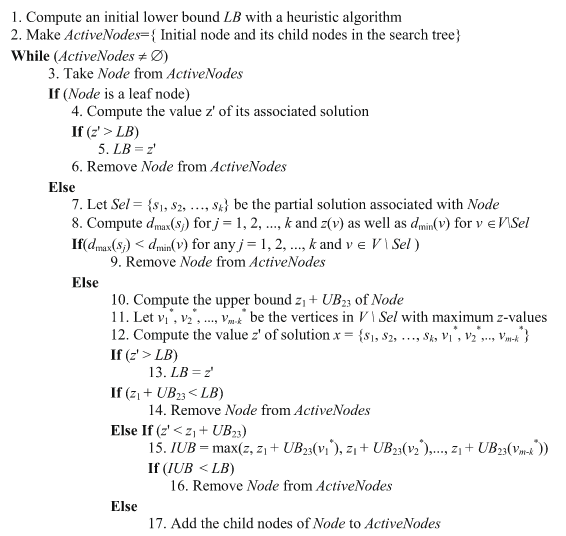
\includegraphics[scale=0.8]{images/RamYPod.png}
    \caption{Pseudocódigo para el algorítmo de ramificación y poda usado en un articulo de Elsevier, el cual se incluye en la bibliografía por si resulta de interés}
    \label{fig:RYP}
\end{figure}

%%%%%%%%%%%%%%%%%%%%%%%%%%%%%%%%%%%%%%%%%%%%%%%%%%%%%%%%%
\newpage{\pagestyle{empty}}
\thispagestyle{empty}

\chapter{\LARGE Experimentos y resultados computacionales}
\label{chapter:resultados}

%%%%%%%%%%%%%%%%%%%%%%%%%%%%%%%%%%%%%%%%%%%%%%%%%%%%%%%%%%%%%%
%%%%%%%%%%%%%%%%%%%%%%%%%%%%%%%%%%%%%%%%%%%%%%%%%%%%%%%%%%%%%%
\section{Constructivo voraz}



%%%%%%%%%%%%%%%%%%%%%%%%%%%%
   \begin{table}[h]
   {\small
   \begin{center}
   \begin{tabular}{cccccc}
      \multicolumn{6}{c}{Algoritmo voraz} \\
      \hline
      Problema & $n$ & $m$ &  Ejecuci\'on & $TCT$ & $CPU(ms)$ \\
      \hline
      I40j_2m_S1_1.txt & 40 & 2 & 1 & 13821 & 1515 \\
      I40j_4m_S1_1.txt & 40 & 4 & 2 & 7353 & 2598 \\
      I40j_6m_S1_1.txt & 40 & 6 & 3 & 5487 & 3494 \\
      I40j_8m_S1_1.txt & 40 & 8 & 4 & 4447 & 5419 \\     
      \hline
   \end{tabular}
   \end{center}
   }
   \caption{Algoritmo voraz. Tabla de resultados}
   \end{table}


   
%%%%%%%%%%%%%%%%%%%%%%%%%%%%%%%%%%%%%%%%%%%%%%%%%%%%%%%%%%%%%%
%%%%%%%%%%%%%%%%%%%%%%%%%%%%%%%%%%%%%%%%%%%%%%%%%%%%%%%%%%%%%%
\section{GRASP}

En el caso a continuación se emplearon todas las busquedas locales, ejecutadas todas una tras otra sobre la S inicial para obtener el mejor resultado de estas. Se muestran ejecuciones con distintos valores de |LRC|.
\\
\\
Se puede apreciar una mejora respecto a la calidad de la solución comparando estos con los obtenidos por el Voraz, aunque esto no siempre se garantiza y en muchos casos se mantiene muy cerca de este.

\clearpage

   \begin{table}[h]
   {\small
   \begin{center}
   \begin{tabular}{ccccccc}
      \multicolumn{7}{c}{GRASP} \\
      \hline
      Problema & $n$ & $m$ & |LRC| & Ejecuci\'on & $TCT$ & $CPU(ms)$ \\
      \hline
      I40j_2m_S1_1.txt & 40 & 2 & 2 & 1 & 13179 & 297391 \\
      I40j_4m_S1_1.txt & 40 & 4 & 2 & 2 & 7243 & 339764 \\
      I40j_6m_S1_1.txt & 40 & 6 & 2 & 3 & 5281 & 308509 \\
      I40j_8m_S1_1.txt & 40 & 8 & 2 & 4 & 4294 & 326351 \\
      I40j_2m_S1_1.txt & 40 & 2 & 3 & 1 & 13604 & 424285 \\
      I40j_4m_S1_1.txt & 40 & 4 & 3 & 2 & 7242 & 377835 \\
      I40j_6m_S1_1.txt & 40 & 6 & 3 & 3 & 5313 & 371937 \\
      I40j_8m_S1_1.txt & 40 & 8 & 3 & 4 & 4339 & 376899 \\
      I40j_2m_S1_1.txt & 40 & 2 & 4 & 1 & 13364 & 483051 \\
      I40j_4m_S1_1.txt & 40 & 4 & 4 & 2 & 7357 & 486922 \\
      I40j_6m_S1_1.txt & 40 & 6 & 4 & 3 & 5278 & 428305 \\
      I40j_8m_S1_1.txt & 40 & 8 & 4 & 4 & 4351 & 437327 \\
      \hline
   \end{tabular}
   \end{center}
   }
   \caption{GRASP. Tabla de resultados}
   \end{table}



%%%%%%%%%%%%%%%%%%%%%%%%%%%%%%%%%%%%%%%%%%%%%%%%%%%%%%%%%%%%%%
%%%%%%%%%%%%%%%%%%%%%%%%%%%%%%%%%%%%%%%%%%%%%%%%%%%%%%%%%%%%%%
\section{GVNS}

Como se puede apreciar, los resultados aqui ya empiezan a mejorar significativamente sobre los encontrados en el Voraz o el GRASP. Aunque esto viene a un coste mucho más elevado, tardandose para estos ejemplos relativamente simples entre 10 y 35 segundos (mientras que todos los casos del grasp se mantenian por debajo de 1)

   \begin{table}[htbp]
   {\small
   \begin{center}
   \begin{tabular}{cccccccc}
      \multicolumn{8}{c}{VNS} \\
      \hline
      Problema & $n$ & $m$ & |LCR| & $k_{max}$ & Ejecuci\'on & $TCT$ & $CPU(ms)$ \\
      \hline   
      I40j_2m_S1_1.txt & $40$ & $2$ & $2$ & $3$ & $1$ & $12869$ & $9825768$ \\
      I40j_4m_S1_1.txt & $40$ & $4$ & $2$ & $3$ & $2$ & $6994$ & $10200866$ \\
      I40j_6m_S1_1.txt & $40$ & $6$ & $2$ & $3$ & $3$ & $5123$ & $11083254$ \\
      I40j_8m_S1_1.txt & $40$ & $8$ & $2$ & $3$ & $4$ & $4147$ & $11883723$ \\
      I40j_2m_S1_1.txt & $40$ & $2$ & $2$ & $5$ & $1$ & $12826$ & $15920742$ \\
      I40j_4m_S1_1.txt & $40$ & $4$ & $2$ & $5$ & $2$ & $6958$ & $18411219$ \\
      I40j_6m_S1_1.txt & $40$ & $6$ & $2$ & $5$ & $3$ & $5088$ & $19760014$ \\
      I40j_8m_S1_1.txt & $40$ & $8$ & $2$ & $5$ & $4$ & $4135$ & $22593976$ \\
      I40j_2m_S1_1.txt & $40$ & $2$ & $2$ & $7$ & $1$ & $12854$ & $22894786$ \\
      I40j_4m_S1_1.txt & $40$ & $4$ & $2$ & $7$ & $2$ & $6990$ & $25807515$ \\
      I40j_6m_S1_1.txt & $40$ & $6$ & $2$ & $7$ & $3$ & $5093$ & $29497841$ \\
      I40j_8m_S1_1.txt & $40$ & $8$ & $2$ & $7$ & $4$ & $4142$ & $31742390$ \\
      I40j_2m_S1_1.txt & $40$ & $2$ & $3$ & $3$ & $1$ & $12959$ & $9965562$ \\
      I40j_4m_S1_1.txt & $40$ & $4$ & $3$ & $3$ & $2$ & $7064$ & $11173606$ \\
      I40j_6m_S1_1.txt & $40$ & $6$ & $3$ & $3$ & $3$ & $5116$ & $12891138$ \\
      I40j_8m_S1_1.txt & $40$ & $8$ & $3$ & $3$ & $4$ & $4149$ & $12334810$ \\
      I40j_2m_S1_1.txt & $40$ & $2$ & $3$ & $5$ & $1$ & $12858$ & $17201037$ \\
      I40j_4m_S1_1.txt & $40$ & $4$ & $3$ & $5$ & $2$ & $6977$ & $18433506$ \\
      I40j_6m_S1_1.txt & $40$ & $6$ & $3$ & $5$ & $3$ & $5106$ & $21373970$ \\
      I40j_8m_S1_1.txt & $40$ & $8$ & $3$ & $5$ & $4$ & $4157$ & $20138231$ \\
      I40j_2m_S1_1.txt & $40$ & $2$ & $3$ & $7$ & $1$ & $12867$ & $24518749$ \\
      I40j_4m_S1_1.txt & $40$ & $4$ & $3$ & $7$ & $2$ & $7006$ & $26315639$ \\
      I40j_6m_S1_1.txt & $40$ & $6$ & $3$ & $7$ & $3$ & $5090$ & $29011823$ \\
      I40j_8m_S1_1.txt & $40$ & $8$ & $3$ & $7$ & $4$ & $4141$ & $34848217$ \\
      I40j_2m_S1_1.txt & $40$ & $2$ & $4$ & $3$ & $1$ & $12816$ & $10678527$ \\
      I40j_4m_S1_1.txt & $40$ & $4$ & $4$ & $3$ & $2$ & $7046$ & $11020342$ \\
      I40j_6m_S1_1.txt & $40$ & $6$ & $4$ & $3$ & $3$ & $5118$ & $12554915$ \\
      I40j_8m_S1_1.txt & $40$ & $8$ & $4$ & $3$ & $4$ & $4165$ & $13431885$ \\
      I40j_2m_S1_1.txt & $40$ & $2$ & $4$ & $5$ & $1$ & $12791$ & $17434455$ \\
      I40j_4m_S1_1.txt & $40$ & $4$ & $4$ & $5$ & $2$ & $7012$ & $20439771$ \\
      I40j_6m_S1_1.txt & $40$ & $6$ & $4$ & $5$ & $3$ & $5101$ & $22921831$ \\
      I40j_8m_S1_1.txt & $40$ & $8$ & $4$ & $5$ & $4$ & $4134$ & $23622101$ \\
      I40j_2m_S1_1.txt & $40$ & $2$ & $4$ & $7$ & $1$ & $12898$ & $23335267$ \\
      I40j_4m_S1_1.txt & $40$ & $4$ & $4$ & $7$ & $2$ & $6983$ & $25236654$ \\
      I40j_6m_S1_1.txt & $40$ & $6$ & $4$ & $7$ & $3$ & $5108$ & $30638487$ \\
      I40j_8m_S1_1.txt & $40$ & $8$ & $4$ & $7$ & $4$ & $4142$ & $32187295$ \\
      \hline
   \end{tabular}
   \end{center}
   }
   \caption{GVNS. Tabla de resultados}
   \end{table}

\end{enumerate}



%%%%%%%%%%%%%%%%%%%%%%%%%%%%%%%%%%%%%%%%%%%%%%%%%%%%%%%%%
\newpage{\pagestyle{empty}}
\thispagestyle{empty}

\chapter{\LARGE Conclusiones y trabajo futuro}
\label{chapter:conclusiones}

Una de las cosas que más se puede apreciar tras llevar a cabo el proyecto es la importancia que se le debe dar a la discusión entre optimización y tiempo de ejecución. Hasta que punto estamos disponibles a optimizar nuestra solución y cuando el tiempo empleado sobrepasa los beneficios obtenidos. 
\\
\\
EL GNVS es un ejemplo muy bueno de esto ya que es obvio desde el principio que supera los algoritmos previo a ello, pero encontrar ese punto medio, ese balance, de calidad de solución frente a tiempo de cálculo es una cuestión importante.

%%%%%%%%%%%%%%%%%%%%%%%%%%%%%%%%%%%%%%%%%%%%%%%%%%%%%%%%%
\newpage{\pagestyle{empty}}
\thispagestyle{empty}

%%%%%%%%%%%%%%%%%%%%%%%%%%%%%%%%%%%%%%%%%%%%%%%%%%%%%%%%%
%\newpage{\pagestyle{empty}\cleardoublepage}
%\thispagestyle{empty}

%\begin{appendix}

%\chapter{\LARGE Título del Apéndice 1}
%\label{appendix:1}
%\input{apendice1.tex}

%\chapter{\LARGE Título del Apéndice 2}
%\label{appendix:2}
%\input{apendice2.tex}

%\end{appendix}

%%%%%%%%%%%%%%%%%%%%%%%%%%%%%%%%%%%%%%%%%%%%%%%%%%%%%%%%%%
\bibliographystyle{plain}
\bibliography{bibliografia}
%%%%%%%%%%%%%%%%%%%%%%%%%%%%%%%%%%%%%%%%%%%%%%%%%%%%%%%%%%

\end{document}
